\subsection{Requerimientos extraídos}

Como se ha establecido en la memoria el proyecto gira en torno a tres
ejes fundamentales:
\begin{itemize}
  \item Proporcionar un lenguaje que facilite la creación de robots.
  \item Ofrecer aAUTOMATOR como servicio.
  \item Ofrecer librerías que consuman dicho servicio.
\end{itemize}

A continuación nos adentraremos en las características y necesidades
que plantea cada elemento.

\subsubsection[Lenguaje robots]{Lenguaje para facilitar la creación de
  robots} Como se ha podido comprobar en Formato
\label{requisitos_lenguaje_robots}
almacenamiento~\ref{formato_almacenamiento},
pág.~\pageref{formato_almacenamiento}, el formato almacenamiento
empleado no facilita la creación y edición directa de robots por parte
de programadores. Si bien nada impide la edición o creación del XML
del robot directamente, cuenta con numerosas desventajas:

\begin{itemize}
  \item Gran redundancia. La naturaleza del XML ocasiona que haya una
    gran serie de elementos repetidos y en general mucho ruido
    sintáctico.
  \item La sintaxis XML es de propósito general. XML se puede usar
    para casi cualquier problema de codificación de datos, pero esto
    conlleva el coste de que no esté optimizado para ningún problema
    en concreto. Para cualquier uso de XML normalmente siempre se puede
    definir un formato más adecuado para ese uso concreto.
\end{itemize}

En general podríamos decir que el XML nos ofrece una solución
inmediata pero que dista de ser la ideal. Consideramos que como
formato de almacenamiento y de entrada a aAUTOMATOR su uso es
adecuado, pero no para ser editado por programadores. Por tanto se ha
decidido hacer un esfuerzo para crear un lenguaje de propósito
específico. Este lenguaje deberá ser traducido al XML. Así podemos
definir el nuevo lenguaje manteniendo aAUTOMATOR intacto.

Es preciso que el nuevo lenguaje tenga una serie de características, de
más a menos importantes:

\begin{enumerate}
  \item Fácil lectura. Un vistazo por parte de un programador
    familiarizado con aAUTOMATOR debería servir para hacerse una idea
    de su estructura.
  \item Concisión. Debe permitir una fácil escritura, sin redundancias
    innecesarias.
  \item Fácil de procesar. El lenguaje ha de poder ser procesado de
    una manera relativamente sencilla. Este requerimiento es menor que
    los dos anteriores y puede ser sacrificado a la hora de alcanzar
    los dos primeros objetivos.
\end{enumerate}

\subsubsection{aAUTOMATOR como servicio}

Otra necesidad es poder ofrecer aAUTOMATOR como servicio. Hasta ahora
aAUTOMATOR sólo se podía invocar desde programas Java. Esto limita el
número de usuarios técnicos y programadores que se pueden beneficiar
de aAUTOMATOR.

El servicio debe estar orientado en primer lugar a programadores y
usuarios técnicos. Como posible ampliación existe la posibilidad de
hacer un \emph{mashup} orientado a usuarios finales. La idea es que
dado el servicio con su documentación asociada un programador pueda
consumir el servicio en su plataforma sin mayor dificultad.

Dada esta necesidad, se ha llegado a la conclusión que exponer el
servicio vía HTTP nos permite alcanzar el mayor número de plataformas
con el menor coste. Existen librerías para acceder HTTP en todas las
plataformas que se precien. Además, al contrario que otros protocolos
de red, no suele ser afectado por la presencia de
\emph{firewalls}. Por tanto, en el presente proyecto aAUTOMATOR ha de
exponerse como un servicio web que pueda ser consumido por numerosas
plataformas.

No conocemos a priori la demanda que pudiera existir por el servicio
ofrecido. Por lo tanto, es necesario que el servicio ofrecido pueda
escalar desde unos pocos usuarios simultáneos a un número elevado
simplemente añadiendo nuevos nodos. Plataformas como
AWS \footnote{\emph{Amazon Web Services}} nos ofrece la posibilidad de
añadir más o menos nodos dinámicamente en función de las necesidades.

El servicio ofrecido debe, pues, poder ejecutarse desde un simple nodo
hasta en un cluster de computadoras.

Además se ha llegado a la conclusión que el servicio debe ofrecer dos
tipos de ejecución:

\begin{description}
  \item[Ejecución síncrona] El programador requiere la ejecución
    inmediata de un robot con un vector de entradas, una vez el
    resultado esté disponible se devuelve inmediatamente al consumidor
    del servicio.
  \item[Ejecución periódica] El programador reclama la ejecución del
    robot con un vector de entradas. A mayores especifica un
    periodo. El robot se ejecutará cada vez que ese periodo de tiempo
    haya transcurrido. El usuario podrá obtener el último resultado
    obtenido. Hemos decidido incluir este tipo de ejecución porque
    creemos que facilita en gran medida muchos casos de uso de
    aAUTOMATOR.

\end{description}

\subsubsection{Librerías}

Para comprobar que el servicio se pueda consumir con facilidad, hemos
de crear varias librerías que sirvan de prueba de concepto. Además, se
priorizarán plataformas que puedan aportar tanto mayor facilidad de
uso o más difusión a aAUTOMATOR.

Una de las librerías ha de ejecutarse sobre la plataforma Java. Java
está instalado en un gran número de sistemas y goza de gran
popularidad entre los programadores. Además la comunidad inicial de
usuarios de aAUTOMATOR son usuarios de esta plataforma. Por lo tanto,
la librería Java gozará de prioridad.

Otra librería ha de hacerse en Python\cite{PYTHON}. Python es un
lenguaje de propósito general con una sintaxis de fácil
lectura. Creemos que es útil hacer una librería en Python porque es un
lenguaje que está gozando de popularidad creciente y está instalado en
la mayoría de sistemas UNIX\cite{UNIX}. Además es un lenguaje que nos
permite ofrecer ejemplos del funcionamiento de la librería de una
manera más directa y sencilla que en el caso de Java.

Además creemos conveniente crear una aplicación de línea de comandos
relativamente amigable. Con ella podremos hacer pruebas y demostrar el
funcionamiento de aAUTOMATOR de manera clara, directa y sencilla. Así
se posibilitará el uso de aAUTOMATOR por parte de usuarios
expertos.

\subsection{Introducción Casos Uso}

En este apartado se mostrarán los casos de uso identificados. Se han
agrupado en dos apartados: \emph{Casos Uso
  Principales}~\ref{casos_uso_principales_section},
pág.~\pageref{casos_uso_principales_section}, y \emph{Casos Uso de
  Aplicación Línea Comandos}~\ref{casos_uso_cli_section},
pág.~\pageref{casos_uso_cli_section}. En este último apartado se
emplea el actor externo \emph{Servicio}. Realmente formaría parte del
proyecto, pero ajustándonos a la Aplicación Línea Comandos es un actor
externo.

Nos hemos decantado por esta agrupación por ninguna razón en especial,
salvo claridad expositiva.

Para empezar, identificaremos y describiremos los actores del
sistema.

\subsection{Actores sistema}

Hemos encontrado los siguientes actores externos a todas las partes
del proyecto:

\subsubsection{Programador}
Se trata de un programador que está familiarizado con aAUTOMATOR y el
lenguaje creado en el presente proyecto. Puede ejecutar directamente
un Robot especificado en el lenguaje creado o convertirlo al XML de
aAUTOMATOR.

Desea extraer información estructurada de la web ya sea para cubrir
una necesidad personal o por encargo. Uno de los objetivos
fundamentales del proyecto es facilitar el uso de aAUTOMATOR por parte
del \emph{Programador} en la medida de lo posible.

\subsubsection{Consumidor Servicio}
Se trata de un cliente que utiliza el protocolo HTTP para acceder y
consumir el servicio. Podría ser una aplicación web o una librería.

\subsubsection{Librería}
Es un caso concreto de \emph{Consumidor de Servicio}. Se trataría de
una librería especialmente creada para simplificar el uso del servicio
desde un lenguaje de programación.

\subsubsection{aAUTOMATOR Runtime}
Es el \emph{runtime} de aAUTOMATOR. Recibe robots especificados en
XML, más un vector de entradas y produce el resultado siguiendo el
funcionamiento especificado. Ver~\ref{COMPORTAMIENTO_AUTOMATOR},
pág.~\pageref{COMPORTAMIENTO_AUTOMATOR}.

\subsubsection{Usuario Experto}
Se trata de un usuario familiarizado con los conceptos de aAUTOMATOR y
capaz de emplear una interfaz de línea de comandos. La interfaz de
línea de comandos debería ofrecer la funcionalidad de aAUTOMATOR de
una manera efectiva.

\subsection{Casos Uso Principales}
\label{casos_uso_principales_section}

\begin{landscape}
\begin{figure}[p]
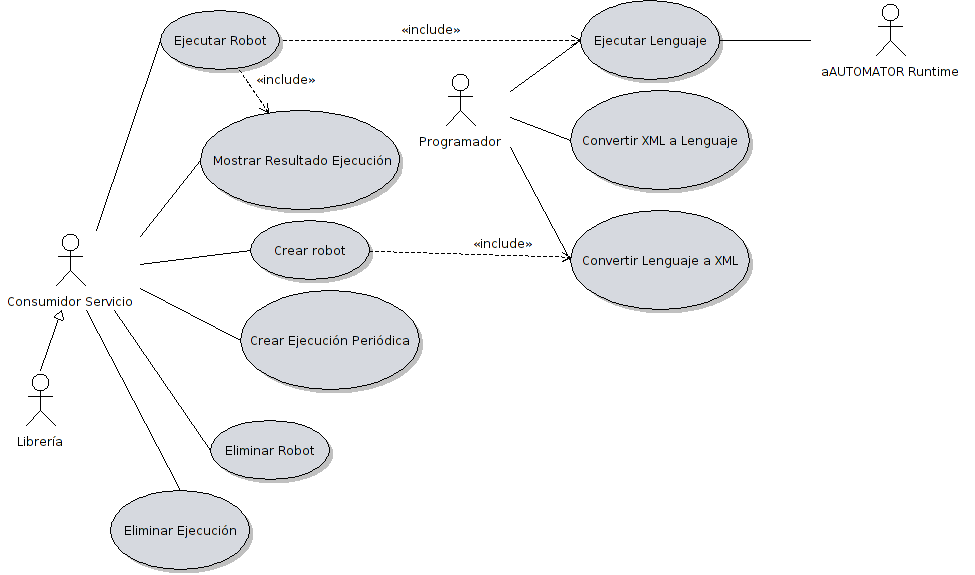
\includegraphics[width=1.4\textwidth]{chapters/technical-manual/diagrams/principal_usecases.violet.png}
\caption{Diagrama Casos Usos principales}\label{casos_uso_principales}
\end{figure}
\end{landscape}

\subsubsection{\large{Caso de uso: Ejecutar Lenguaje}}
\label{ejecutar_lenguaje_caso_uso_minilenguaje}

\begin{tabular}[h]{ p{.3\textwidth } p{.7\textwidth }}

\textbf{Descripción} & El sistema ejecuta el robot especificado en el
lenguaje creado por el proyecto. El lenguaje ha de tener las
características establecidas en \ref{requisitos_lenguaje_robots},
pág.~\pageref{requisitos_lenguaje_robots}.\\[3mm]

\textbf{Actores} & Programador, aAUTOMATOR \emph{Runtime}.\\[3mm]

\textbf{Precondiciones} & - \\[3mm]

\textbf{Postcondiciones} & - \\[3mm]

\textbf{Flujo principal} & \begin{enumerate}[leftmargin=1em,topsep=0pt, partopsep=0pt]
  \item El programador crea o edita un robot en el lenguaje definido
    por el proyecto.
  \item El sistema transforma el lenguaje al XML de
    aAUTOMATOR. [\emph{Excepción A}]
  \item El sistema solicita al aAUTOMATOR \emph{Runtime} que se
    ejecute con un vector de entradas proporcionado por el
    programador. [\emph{Excepción B}]
  \item El sistema muestra el resultado al programador.
\end{enumerate}\\[3mm]

\textbf{Flujos alternativos o Excepciones} &
\begin{enumerate}[label=\Alph*:,leftmargin=1em,topsep=0pt, partopsep=0pt]
\item Lenguaje con sintaxis incorrecta
  \begin{enumerate}[label=\arabic*.,topsep=0pt, partopsep=0pt]
    \item Se muestra al programador el error producido.
  \end{enumerate}
\item Error en ejecución aAUTOMATOR
  \begin{enumerate}[label=\arabic*.,topsep=0pt, partopsep=0pt]
    \item Se muestra al programador el error producido.
  \end{enumerate}
\end{enumerate}\\[3mm]
\end{tabular}

\begin{figure}[bp!]
  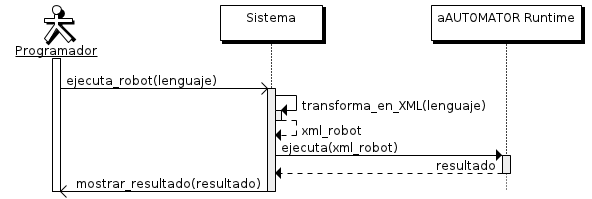
\includegraphics[totalheight=.2\textheight]{chapters/technical-manual/diagrams/sequence/ejecutar_lenguaje.png}
\caption{Ejecutar Lenguaje}\label{ejecutar_lenguaje}
\end{figure}
\clearpage

\subsubsection{\large{Caso de uso: Convertir XML a Lenguaje}}

\begin{tabular}[h]{ p{.3\textwidth } p{.7\textwidth }}

\textbf{Descripción} & Tomar el XML de aAUTOMATOR
~\ref{formato_almacenamiento}, pág.~\pageref{formato_almacenamiento}
y convertirlo en lenguaje. Esto es especialmente útil para la
herramienta visual, permitiendo ver la definición en el lenguaje del
robot que está siendo creado.\\[3mm]

\textbf{Actores} & Programador.\\[3mm]

\textbf{Precondiciones} & - \\[3mm]

\textbf{Postcondiciones} & - \\[3mm]

\textbf{Flujo principal} & \begin{enumerate}[leftmargin=1em,topsep=0pt, partopsep=0pt]
  \item El programador proporciona un XML de aAUTOMATOR válido. [\emph{Excepción A}]
  \item El sistema muestra el lenguaje creado.
\end{enumerate}\\[3mm]

\textbf{Flujos alternativos o Excepciones} &
\begin{enumerate}[label=\Alph*:,leftmargin=1em,topsep=0pt, partopsep=0pt]
\item XML de aAUTOMATOR incorrecto
  \begin{enumerate}[label=\arabic*.,topsep=0pt, partopsep=0pt]
    \item Se muestra al programador el error de formato existente.
  \end{enumerate}
\end{enumerate}\\[3mm]
\end{tabular}

\begin{figure}[bp!]
  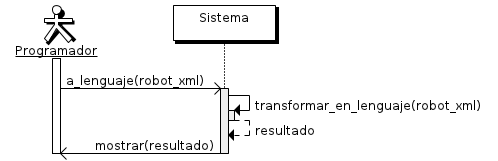
\includegraphics[width=1\textwidth]{chapters/technical-manual/diagrams/sequence/convertir_xml_a_lenguaje.png}
\caption{Convertir XML a Lenguaje}
\end{figure}
\clearpage

\subsubsection{\large{Caso de uso: Convertir Lenguaje a XML}}
\label{convertir_lenguaje_a_xml_caso_uso}
\begin{tabular}[h]{ p{.3\textwidth } p{.7\textwidth }}

\textbf{Descripción} & El sistema convierte el robot especificado en
el lenguaje creado al formato XML soportado por
aAUTOMATOR. Ver~\ref{formato_almacenamiento},
pág.~\pageref{formato_almacenamiento}. \\[3mm]

\textbf{Actores} & Programador.\\[3mm]

\textbf{Precondiciones} & - \\[3mm]

\textbf{Postcondiciones} & - \\[3mm]

\textbf{Flujo principal} & \begin{enumerate}[leftmargin=1em,topsep=0pt, partopsep=0pt]
  \item El programador crea o edita un robot en el lenguaje definido
    por el proyecto.
  \item El sistema transforma el lenguaje al XML de
    aAUTOMATOR. [\emph{Excepción A}]
\end{enumerate}\\[3mm]

\textbf{Flujos alternativos o Excepciones} &
\begin{enumerate}[label=\Alph*:,leftmargin=1em,topsep=0pt,
    partopsep=0pt]
\item Lenguaje con sintaxis incorrecta
  \begin{enumerate}[label=\arabic*.,topsep=0pt, partopsep=0pt]
    \item Se muestra al programador el error producido.
  \end{enumerate}
\end{enumerate}\\[3mm]
\end{tabular}

\begin{figure}[bp!]
  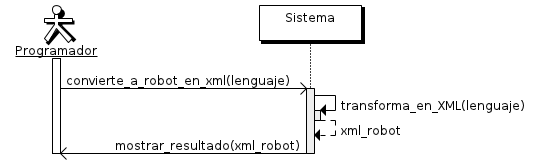
\includegraphics[width=1\textwidth]{chapters/technical-manual/diagrams/sequence/convertir_lenguaje_a_xml.png}
\caption{Convertir Lenguaje a XML}
\end{figure}
\clearpage

\subsubsection{\large{Caso de uso: Mostrar Resultado Ejecución}}
\label{mostrar_resultado_ejecucion_servicio}
\begin{tabular}[h]{ p{.3\textwidth } p{.7\textwidth }}

\textbf{Descripción} & Muestra el resultado de una ejecución. Debe
contener datos como el vector de salida, la fecha en la que se ha
llevado a cabo, el tiempo transcurrido en la ejecución y una
referencia al robot a partir del cual ha sido creada.\\[3mm]

\textbf{Actores} & Consumidor Servicio (p.~ej.: Librería).\\[3mm]

\textbf{Precondiciones} & - \\[3mm]

\textbf{Postcondiciones} & - \\[3mm]

\textbf{Flujo principal} & \begin{enumerate}[leftmargin=1em,topsep=0pt, partopsep=0pt]
  \item El consumidor del servicio accede a una URL que referencia una
    ejecución. [\emph{Excepción A}]
  \item El sistema devuelve información sobre la ejecución.
\end{enumerate}\\[3mm]

\textbf{Flujos alternativos o Excepciones} &
\begin{enumerate}[label=\Alph*:,leftmargin=1em,topsep=0pt, partopsep=0pt]
\item No existe ejecución con ese código
  \begin{enumerate}[label=\arabic*.,topsep=0pt, partopsep=0pt]
    \item Mostrar error indicando que no existe ejecución con ese
      código.
  \end{enumerate}
\end{enumerate}\\[3mm]
\end{tabular}

\begin{figure}[bp!]
  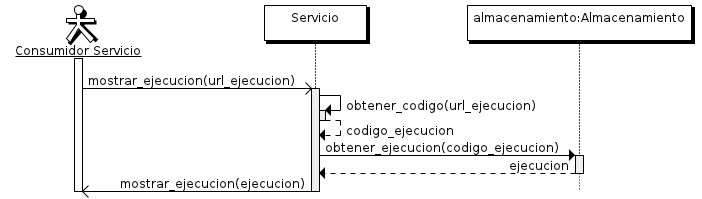
\includegraphics[width=1\textwidth]{chapters/technical-manual/diagrams/sequence/mostrar_resultado_ejecucion.png}
\caption{Mostrar Resultado Ejecución}
\end{figure}
\clearpage

\subsubsection{\large{Caso de uso: Ejecutar Robot}}

\begin{tabular}[h]{ p{.3\textwidth } p{.7\textwidth }}

\textbf{Descripción} & Se indica un robot y un vector de entrada con
el que ejecutarlo. Con esta información se puede realizar una
ejecución del robot en aAUTOMATOR siguiendo
\ref{ejecutar_lenguaje_caso_uso_minilenguaje},
pág.~\pageref{ejecutar_lenguaje_caso_uso_minilenguaje}. Una vez
  finalizada se muestra el resultado al consumidor del servicio
  siguiendo \ref{mostrar_resultado_ejecucion_servicio},
  pág.~\pageref{mostrar_resultado_ejecucion_servicio}\\[3mm]

\textbf{Actores} & Consumidor Servicio (p.~ej.: Librería).\\[3mm]

\textbf{Precondiciones} & - \\[3mm]

\textbf{Postcondiciones} & Existe una nueva ejecución \\[3mm]

\textbf{Flujo principal} & \begin{enumerate}[leftmargin=1em,topsep=0pt, partopsep=0pt]
  \item El Consumidor Servicio indica el código del robot que se
    quiere ejecutar más un vector de entradas. [\emph{Excepción A}]
  \item El robot especificado se ejecuta por aAUTOMATOR
    \emph{Runtime},
    ver~\pageref{ejecutar_lenguaje_caso_uso_minilenguaje}.
    [\emph{Excepción B}]
  \item El resultado obtenido se muestra al Consumidor del
    Servicio. Ver~\ref{mostrar_resultado_ejecucion_servicio}.
\end{enumerate}\\[3mm]

\textbf{Flujos alternativos o Excepciones} &
\begin{enumerate}[label=\Alph*:,leftmargin=1em,topsep=0pt,
    partopsep=0pt]
\item El robot no existe
  \begin{enumerate}[label=\arabic*.,topsep=0pt, partopsep=0pt]
    \item Se deniega la petición indicando la causa.
  \end{enumerate}
\item Error ejecución aAUTOMATOR
  \begin{enumerate}[label=\arabic*.,topsep=0pt, partopsep=0pt]
     \item El resultado mostrado contendrá una descripción del error
       en vez de un resultado convencional.
  \end{enumerate}
\end{enumerate}\\[3mm]
\end{tabular}

\begin{figure}[bp!]
  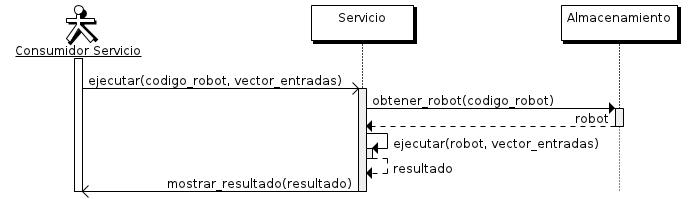
\includegraphics[width=1\textwidth]{chapters/technical-manual/diagrams/sequence/ejecutar_robot.png}
\caption{Ejecutar Robot}
\end{figure}
\clearpage

\subsubsection{\large{Caso de uso: Crear Robot}}

\begin{tabular}[h]{ p{.3\textwidth } p{.7\textwidth }}

\textbf{Descripción} & Crear y almacenar un Robot en el sistema a
partir de un robot tanto en XML como en el lenguaje definido en este
proyecto. \\[3mm]

\textbf{Actores} & Consumidor Servicio (p.~ej.: Librería).\\[3mm]

\textbf{Precondiciones} & - \\[3mm]

\textbf{Postcondiciones} & Se almacena un Robot en el sistema pudiendo
ser referenciado posteriormente. \\[3mm]

\textbf{Flujo principal} & \begin{enumerate}[leftmargin=1em,topsep=0pt, partopsep=0pt]
  \item El \emph{Consumidor Servicio} hace una petición que incluye un robot
    de aAUTOMATOR en XML o en el lenguaje definido en este
    proyecto. [\emph{Excepción A}]
  \item Si el robot no está especificado en XML se convierte al
    mismo. Ver \ref{convertir_lenguaje_a_xml_caso_uso},
    pág.~\pageref{convertir_lenguaje_a_xml_caso_uso}.
  \item Se almacena el robot con la información suministrada.
\end{enumerate}\\[3mm]

\textbf{Flujos alternativos o Excepciones} &
\begin{enumerate}[label=\Alph*:,leftmargin=1em,topsep=0pt, partopsep=0pt]
\item Lenguaje con sintaxis incorrecta
  \begin{enumerate}[label=\arabic*.,topsep=0pt, partopsep=0pt]
    \item Se rechaza la petición indicando el error producido.
  \end{enumerate}
\end{enumerate}\\[3mm]
\end{tabular}

\begin{figure}[bp!]
  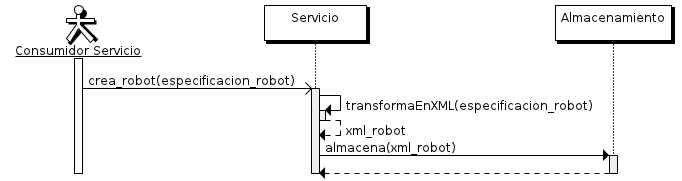
\includegraphics[width=1\textwidth]{chapters/technical-manual/diagrams/sequence/crear_robot.png}
\caption{Crear Robot}
\end{figure}
\clearpage
\subsubsection{\large{Caso de uso: Crear Ejecución Periódica}}

\begin{tabular}[h]{ p{.3\textwidth } p{.7\textwidth }}

\textbf{Descripción} & Crear y almacenar una ejecución periódica a
partir de una referencia a un robot, un periodo de tiempo y un vector
de cadenas de entrada. La ejecución se realizará cada vez que
transcurra el periodo especificado. \\[3mm]

\textbf{Actores} & Consumidor Servicio (p.~ej.: Librería).\\[3mm]

\textbf{Precondiciones} & - \\[3mm]

\textbf{Postcondiciones} & Se realizará la ejecución del robot
referenciado cada vez que transcurra el periodo especificado. El
resultado de la última de estas ejecuciones puede ser mostrado.\\[3mm]

\textbf{Flujo principal} & \begin{enumerate}[leftmargin=1em,topsep=0pt, partopsep=0pt]
  \item El \emph{Consumidor Servicio} hace una petición que referencia
    un robot ya existente, incluye un periodo de tiempo y especifica
    un vector de cadenas de entrada. [\emph{Excepción A}]
  \item Se almacena una ejecución periódica en el sistema de modo que
    se ejecute según el periodo indicado.
\end{enumerate}\\[3mm]

\textbf{Flujos alternativos o Excepciones} &
\begin{enumerate}[label=\Alph*:,leftmargin=1em,topsep=0pt, partopsep=0pt]
\item El periodo es incorrecto.
  \begin{enumerate}[label=\arabic*.,topsep=0pt, partopsep=0pt]
    \item Se deniega la petición indicando la causa.
  \end{enumerate}
\end{enumerate}\\[3mm]
\end{tabular}

\begin{figure}[bp!]
  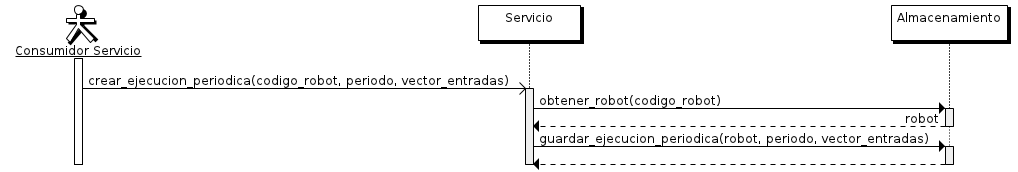
\includegraphics[width=1\textwidth]{chapters/technical-manual/diagrams/sequence/crear_ejecucion_periodica.png}
\caption{Crear Ejecución Periódica}
\end{figure}
\clearpage

\subsubsection{\large{Caso de uso: Eliminar Robot}}

\begin{tabular}[h]{ p{.3\textwidth } p{.7\textwidth }}
\textbf{Descripción} & Elimina un robot existente en el sistema junto
a todos sus datos asociados. \\[3mm]

\textbf{Actores} & Consumidor Servicio (p.~ej.: Librería).\\[3mm]

\textbf{Precondiciones} & - \\[3mm]

\textbf{Postcondiciones} & El robot mas todas sus ejecuciones
asociadas dejan de poder ser referenciados. \\[3mm]

\textbf{Flujo principal} & \begin{enumerate}[leftmargin=1em,topsep=0pt, partopsep=0pt]
  \item El \emph{Consumidor Servicio} hace una petición pidiendo que
    el robot referenciado sea eliminado. [\emph{Excepción A}]
  \item El sistema elimina el robot indicado, junto a las ejecuciones
    asociadas.
\end{enumerate}\\[3mm]

\textbf{Flujos alternativos o Excepciones} &
\begin{enumerate}[label=\Alph*:,leftmargin=1em,topsep=0pt, partopsep=0pt]
\item El Robot no existe.
  \begin{enumerate}[label=\arabic*.,topsep=0pt, partopsep=0pt]
    \item No es necesario hacer nada.
  \end{enumerate}
\end{enumerate}\\[3mm]
\end{tabular}

\begin{figure}[bp!]
  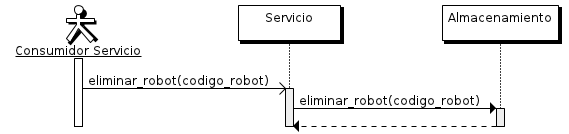
\includegraphics[width=1\textwidth]{chapters/technical-manual/diagrams/sequence/eliminar_robot.png}
\caption{Eliminar Robot}
\end{figure}
\clearpage
\subsubsection{\large{Caso de uso: Eliminar Ejecución}}

\begin{tabular}[h]{ p{.3\textwidth } p{.7\textwidth }}

\textbf{Descripción} &  Elimina una ejecución existente en el sistema. \\[3mm]

\textbf{Actores} & Consumidor Servicio (p.~ej.: Librería).\\[3mm]

\textbf{Precondiciones} & - \\[3mm]

\textbf{Postcondiciones} & La ejecución deja de poder ser referenciada. \\[3mm]

\textbf{Flujo principal} & \begin{enumerate}[leftmargin=1em,topsep=0pt, partopsep=0pt]
  \item El \emph{Consumidor Servicio} hace una petición pidiendo que
    la ejecución referenciada sea eliminada. [\emph{Excepción A}]
  \item El sistema elimina la ejecución indicada.
\end{enumerate}\\[3mm]

\textbf{Flujos alternativos o Excepciones} &
\begin{enumerate}[label=\Alph*:,leftmargin=1em,topsep=0pt, partopsep=0pt]
\item La Ejecución no existe
  \begin{enumerate}[label=\arabic*.,topsep=0pt, partopsep=0pt]
    \item No es necesario hacer nada.
  \end{enumerate}
\end{enumerate}\\[3mm]
\end{tabular}

\begin{figure}[bp!]
  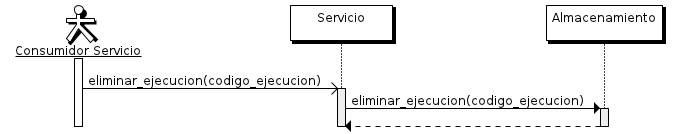
\includegraphics[width=1\textwidth]{chapters/technical-manual/diagrams/sequence/eliminar_ejecucion.png}
\caption{Eliminar Ejecución}
\end{figure}
\clearpage

\subsection{Casos Uso de Aplicación Línea Comandos}
\label{casos_uso_cli_section}
\begin{figure}[p]
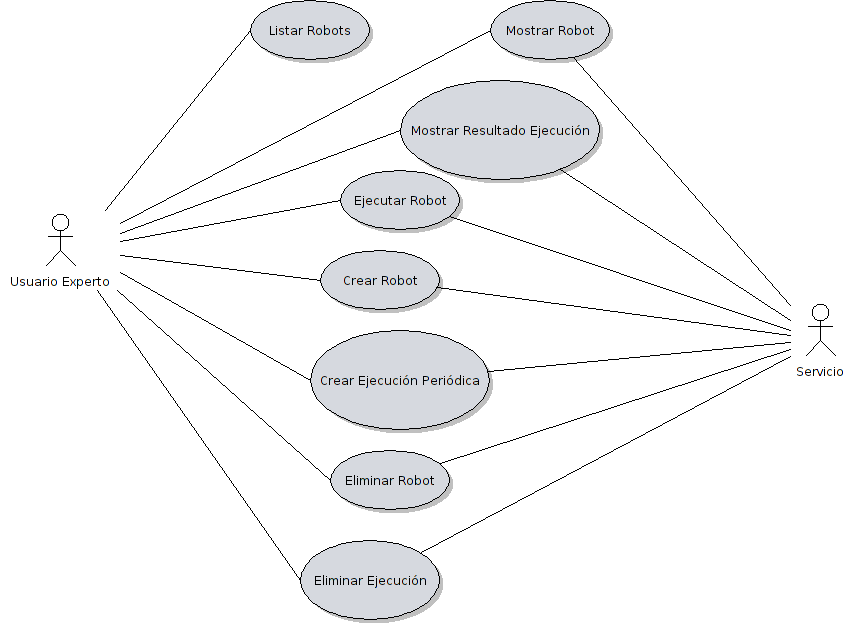
\includegraphics[width=\textwidth]{chapters/technical-manual/diagrams/cli.violet.png}
\caption{Diagrama Casos Usos Línea Comandos}\label{casos_uso_cli}
\end{figure}

\subsubsection{\large{Caso de uso: Listar Robots}}
\label{listar_robots}

\begin{tabular}[h]{ p{.3\textwidth } p{.7\textwidth }}

\textbf{Descripción} & Permite listar los robots creados por un
usuario localmente junto a información asociada. Esto es útil para
facilitar el acceso a los últimos Robots con los que se ha
trabajado.\\[3mm]

\textbf{Actores} & Usuario Experto.\\[3mm]

\textbf{Precondiciones} & - \\[3mm]

\textbf{Postcondiciones} & - \\[3mm]

\textbf{Flujo principal} & \begin{enumerate}[leftmargin=1em,topsep=0pt, partopsep=0pt]
  \item El usuario solicita ver los robots creados desde ese equipo.
  \item El sistema muestra un listado de los robots junto a sus
    ejecuciones asociadas.
\end{enumerate}\\[3mm]

\textbf{Flujos alternativos o Excepciones} &
\end{tabular}

\begin{figure}[bp!]
  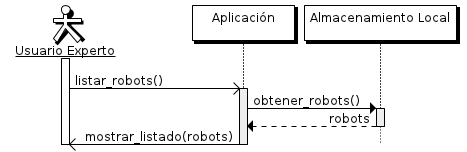
\includegraphics[width=1\textwidth]{chapters/technical-manual/diagrams/sequence/expert_user/listar_robots.png}
\caption{Listar Robots}
\end{figure}
\clearpage
\subsubsection{\large{Caso de uso: Mostrar Robot}}

\begin{tabular}[h]{ p{.3\textwidth } p{.7\textwidth }}

\textbf{Descripción} & Muestra la definición del Robot indicado
accediendo al servicio.\\[3mm]

\textbf{Actores} & Usuario Experto, Servicio.\\[3mm]

\textbf{Precondiciones} & - \\[3mm]

\textbf{Postcondiciones} & - \\[3mm]

\textbf{Flujo principal} & \begin{enumerate}[leftmargin=1em,topsep=0pt, partopsep=0pt]
  \item El usuario indica el código del Robot que quiere mostrar. [\emph{Excepción A}]
  \item Se accede al servicio y se muestra la definición del robot al
    usuario.
\end{enumerate}\\[3mm]

\textbf{Flujos alternativos o Excepciones} &
\begin{enumerate}[label=\Alph*:,leftmargin=1em,topsep=0pt, partopsep=0pt]
\item El robot no existe
  \begin{enumerate}[label=\arabic*.,topsep=0pt, partopsep=0pt]
    \item Se indica al usuario que el robot no existe.
  \end{enumerate}
\end{enumerate}\\[3mm]
\end{tabular}

\begin{figure}[bp!]
  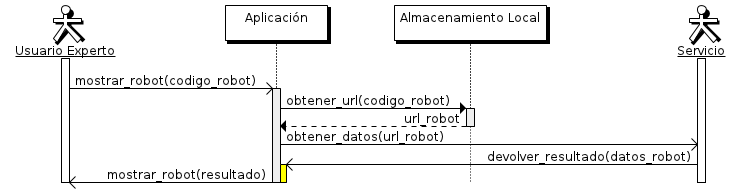
\includegraphics[width=1\textwidth]{chapters/technical-manual/diagrams/sequence/expert_user/mostrar_robot.png}
\caption{Mostrar Robot}
\end{figure}
\clearpage
\subsubsection{\large{Caso de uso: Mostrar Resultado Ejecución}}

\begin{tabular}[h]{ p{.3\textwidth } p{.7\textwidth }}

\textbf{Descripción} & Muestra la definición de la ejecución
especificada accediendo al servicio. \\[3mm]

\textbf{Actores} & Usuario Experto, Servicio.\\[3mm]

\textbf{Precondiciones} & - \\[3mm]

\textbf{Postcondiciones} & - \\[3mm]

\textbf{Flujo principal} & \begin{enumerate}[leftmargin=1em,topsep=0pt, partopsep=0pt]
  \item El usuario indica el código de la Ejecución que quiere mostrar. [\emph{Excepción A}]
  \item La aplicación accede al servicio y se muestran los datos de la
    Ejecución especificada.
\end{enumerate}\\[3mm]

\textbf{Flujos alternativos o Excepciones} &
\begin{enumerate}[label=\Alph*:,leftmargin=1em,topsep=0pt, partopsep=0pt]
\item La Ejecución no existe.
  \begin{enumerate}[label=\arabic*.,topsep=0pt, partopsep=0pt]
    \item Se informa al usuario de la que la ejecución no existe.
  \end{enumerate}
\end{enumerate}\\[3mm]
\end{tabular}

\begin{figure}[bp!]
  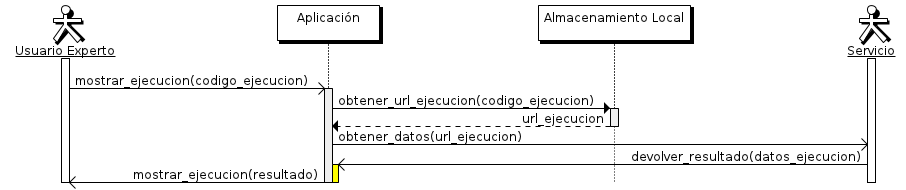
\includegraphics[width=1\textwidth]{chapters/technical-manual/diagrams/sequence/expert_user/mostrar_resultado_ejecucion.png}
\caption{Mostrar Resultado Ejecución}
\end{figure}
\clearpage

\subsubsection{\large{Caso de uso: Ejecutar Robot}}

\begin{tabular}[h]{ p{.3\textwidth } p{.7\textwidth }}

\textbf{Descripción} & Ejecuta el Robot especificado con el vector de
cadenas de entrada especificado. Se comunica con el servicio para
llevarlo a cabo.\\[3mm]

\textbf{Actores} & Usuario Experto, Servicio.\\[3mm]

\textbf{Precondiciones} & - \\[3mm]

\textbf{Postcondiciones} & - \\[3mm]

\textbf{Flujo principal} & \begin{enumerate}[leftmargin=1em,topsep=0pt, partopsep=0pt]
  \item El usuario indica el código del Robot que quiere ejecutar
    junto al vector de cadenas de entrada. [\emph{Excepción A}]
  \item La aplicación accede al servicio y le indica que ha de
    realizar una ejecución con el robot especificado y el vector de
    cadenas de entrada.
\end{enumerate}\\[3mm]

\textbf{Flujos alternativos o Excepciones} &
\begin{enumerate}[label=\Alph*:,leftmargin=1em,topsep=0pt, partopsep=0pt]
\item No existe un Robot con ese código.
  \begin{enumerate}[label=\arabic*.,topsep=0pt, partopsep=0pt]
    \item Se indica al usuario que el robot no existe.
  \end{enumerate}
\end{enumerate}\\[3mm]
\end{tabular}

\begin{figure}[bp!]
  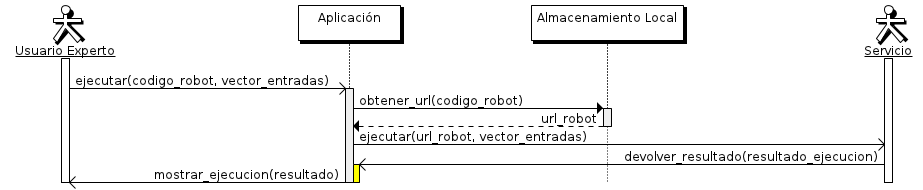
\includegraphics[width=1\textwidth]{chapters/technical-manual/diagrams/sequence/expert_user/ejecutar_robot.png}
\caption{Ejecutar Robot}
\end{figure}
\clearpage
\subsubsection{\large{Caso de uso: Crear Robot}}

\begin{tabular}[h]{ p{.3\textwidth } p{.7\textwidth }}

\textbf{Descripción} & Crea un nuevo Robot en el servicio ya sea a
partir del formato XML o del lenguaje definido en este
proyecto.\\[3mm]

\textbf{Actores} & Usuario Experto, Servicio.\\[3mm]

\textbf{Precondiciones} & - \\[3mm]

\textbf{Postcondiciones} & Un nuevo Robot es creado y almacenado en el
Servicio. El Robot creado aparecerá en el listado.\\[3mm]

\textbf{Flujo principal} & \begin{enumerate}[leftmargin=1em,topsep=0pt, partopsep=0pt]
  \item El usuario proporciona el XML o una instancia del lenguaje
    definido.
  \item El servicio crea un nuevo robot a partir de estos
    datos. [\emph{Excepción A}]
  \item Se guarda la URL del robot creado para que pueda ser accedido
    posteriormente por su código.
\end{enumerate}\\[3mm]

\textbf{Flujos alternativos o Excepciones} &
\begin{enumerate}[label=\Alph*:,leftmargin=1em,topsep=0pt, partopsep=0pt]
\item El robot especificado es incorrecto.
  \begin{enumerate}[label=\arabic*.,topsep=0pt, partopsep=0pt]
    \item Se cancela la petición de creación de Robot y se muestra el
      error al usuario.
  \end{enumerate}
\end{enumerate}\\[3mm]
\end{tabular}

\begin{figure}[bp!]
  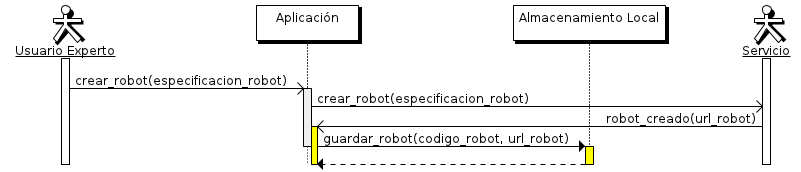
\includegraphics[width=1\textwidth]{chapters/technical-manual/diagrams/sequence/expert_user/crear_robot.png}
\caption{Crear Robot}
\end{figure}
\clearpage
\subsubsection{\large{Caso de uso: Crear Ejecución Periódica}}

\begin{tabular}[h]{ p{.3\textwidth } p{.7\textwidth }}

\textbf{Descripción} & Crea una nueva Ejecución Periódica a partir del
código de un Robot ya existente, un periodo de tiempo y un vector de
cadena de entradas.  La ejecución se realizará cada vez que transcurra
el periodo especificado.\\[3mm]

\textbf{Actores} & Usuario Experto, Servicio.\\[3mm]

\textbf{Precondiciones} & - \\[3mm]

\textbf{Postcondiciones} & Se realizará la ejecución del robot
referenciado en el servicio cada vez que transcurra el periodo
especificado. El resultado de la última de estas ejecuciones puede ser
mostrado. \\[3mm]

\textbf{Flujo principal} & \begin{enumerate}[leftmargin=1em,topsep=0pt, partopsep=0pt]
  \item El usuario indica un el código de un Robot, un periodo de
    tiempo y un vector de cadena de entradas.
  \item El servicio recibe los datos de entrada y crea una ejecución
    periódica. [\emph{Excepción A}]
\end{enumerate}\\[3mm]

\textbf{Flujos alternativos o Excepciones} &
\begin{enumerate}[label=\Alph*:,leftmargin=1em,topsep=0pt, partopsep=0pt]
\item El Robot indicado no existe
  \begin{enumerate}[label=\arabic*.,topsep=0pt, partopsep=0pt]
    \item Se indica la situación al usuario.
  \end{enumerate}
\end{enumerate}\\[3mm]
\end{tabular}

\begin{figure}[bp!]
  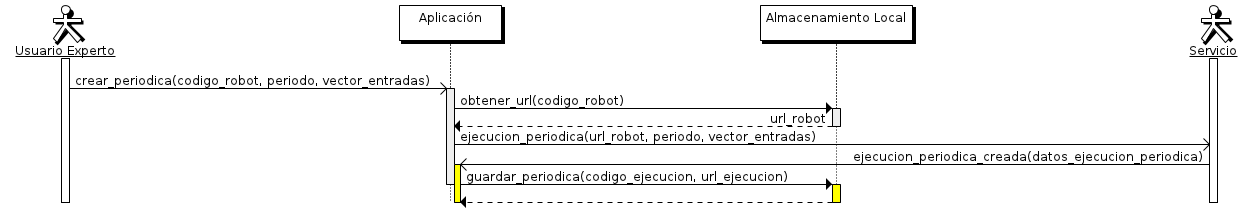
\includegraphics[width=1\textwidth]{chapters/technical-manual/diagrams/sequence/expert_user/crear_ejecucion_periodica.png}
\caption{Crear Ejecución Periódica}
\end{figure}
\clearpage
\subsubsection{\large{Caso de uso: Eliminar Robot}}

\begin{tabular}[h]{ p{.3\textwidth } p{.7\textwidth }}

\textbf{Descripción} & Elimina un robot existente en el sistema junto
a todos sus datos asociados.\\[3mm]

\textbf{Actores} & Usuario Experto, Servicio.\\[3mm]

\textbf{Precondiciones} & - \\[3mm]

\textbf{Postcondiciones} & El robot mas todas sus ejecuciones
asociadas dejan de poder ser referenciados. Tampoco aparecerán en el
listado local Ver \ref{listar_robots},
pág~\pageref{listar_robots}.\\[3mm]

\textbf{Flujo principal} & \begin{enumerate}[leftmargin=1em,topsep=0pt, partopsep=0pt]
  \item El usuario indica el código del Robot que desea eliminar.
  \item Se elimina el Robot indicado, junto a las ejecuciones
    asociadas del almacenamiento local.
  \item El servicio elimina el Robot indicado, junto a las ejecuciones
    asociadas. [\emph{Excepción A}]
\end{enumerate}\\[3mm]

\textbf{Flujos alternativos o Excepciones} &
\begin{enumerate}[label=\Alph*:,leftmargin=1em,topsep=0pt, partopsep=0pt]
\item El Robot no existe.
  \begin{enumerate}[label=\arabic*.,topsep=0pt, partopsep=0pt]
    \item No es necesario hacer nada.
  \end{enumerate}
\end{enumerate}\\[3mm]
\end{tabular}

\begin{figure}[bp!]
  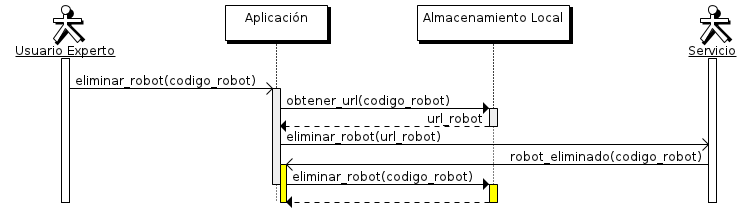
\includegraphics[width=1\textwidth]{chapters/technical-manual/diagrams/sequence/expert_user/eliminar_robot.png}
\caption{Eliminar Robot}
\end{figure}
\clearpage
\subsubsection{\large{Caso de uso: Eliminar Ejecución}}

\begin{tabular}[h]{ p{.3\textwidth } p{.7\textwidth }}

\textbf{Descripción} &  Elimina una ejecución del servicio y
localmente, de modo que no pueda volver a ser accesible. \\[3mm]

\textbf{Actores} & Usuario Experto, Servicio.\\[3mm]

\textbf{Precondiciones} & - \\[3mm]

\textbf{Postcondiciones} & La Ejecución indicada deja de poder ser
referenciada. Tampoco aparecerán en el listado local Ver
\ref{listar_robots}, pág~\pageref{listar_robots}. \\[3mm]

\textbf{Flujo principal} & \begin{enumerate}[leftmargin=1em,topsep=0pt, partopsep=0pt]
  \item El usuario indica el código de la Ejecución que desea
    eliminar.
  \item Se elimina del almacenamiento local la Ejecución indicada.
  \item El servicio elimina la ejecución indicada. [\emph{Excepción A}]
\end{enumerate}\\[3mm]

\textbf{Flujos alternativos o Excepciones} &
\begin{enumerate}[label=\Alph*:,leftmargin=1em,topsep=0pt, partopsep=0pt]
\item La Ejecución no existe.
  \begin{enumerate}[label=\arabic*.,topsep=0pt, partopsep=0pt]
    \item No es necesario hacer nada.
  \end{enumerate}
\end{enumerate}\\[3mm]
\end{tabular}

\begin{figure}[bp!]
  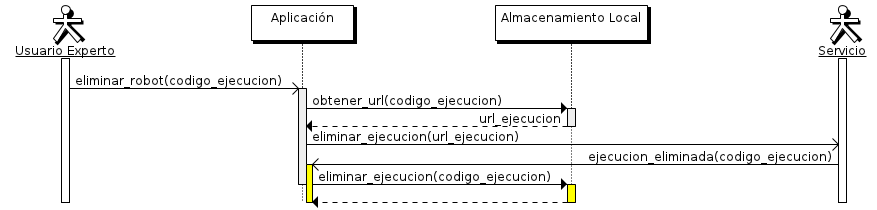
\includegraphics[width=1\textwidth]{chapters/technical-manual/diagrams/sequence/expert_user/eliminar_ejecucion.png}
\caption{Eliminar Ejecución}
\end{figure}
\clearpage
